\input{mmd-article-header}
\def\mytitle{Chapter 2 -- Binding Antibodies to Nanospheres}
\input{mmd-article-begin-doc}
\def\bibliocommand{\bibliography{theis.bib}}
At the end of Summer 2010, Oliver Hoidn and Perry Ellis had determined that the optimal number of OPSS-PEG-antibody (OPAb) molecules per nanosphere was approximately 2000; however, there were significant concerns as to whether the OPSS-PEG-NHS (OPN) was successfully binding to the lysines on the antibody, or whether monolayer formation was simply the result of the antibodies binding to the nanospheres via van der Waals forces. The OPN reacts with a lysine by substituting the nitrogen atom in the NHS ester for the nitrogen atom on the functional group of the lysine (and their respective attached molecules, by proxy). A diagram of this reaction is shown in \autoref{nhsreaction}.

\begin{figure}[htbp]
\centering
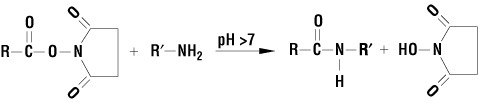
\includegraphics[keepaspectratio,width=\textwidth,height=0.75\textheight]{NHSreaction.jpg}
\caption{Schematic diagram of the OPN+antibody$\to$OPAb reaction. \textbf{R} represents the OPSS-PEG, and \textbf{R'} represents the antibody. The reaction is favored in basic conditions. From ~\citep{nhsreaction}}
\label{nhsreaction}
\end{figure}



Although the reaction requires a basic pH ($>$7) to run, basic conditions also favor a competing reaction, in which hydrolysis occurs and the NHS ester is replaced with a hydroxyl group. This renders the molecule unable to bind to antibodies, and the half-life of the hydrolysis reaction can be on the order of minutes at pH 8~\citep{nhshalflife}. Consequently, there was a concern that a large portion of the OPN used in the OPN+antibody$\to$OPAb reaction was not binding to the antibody.

Fortunately, a direct physical measurement can be used to quantify the hydrolysis of the NHS ester. 

\input{mmd-memoir-footer}

\end{document}
